\section{From orthorombic strained cell to pseudo-hexagonal unit cell} \label{app:ortho2hex}
% \begin{figure}[!h]
%     \centering
%     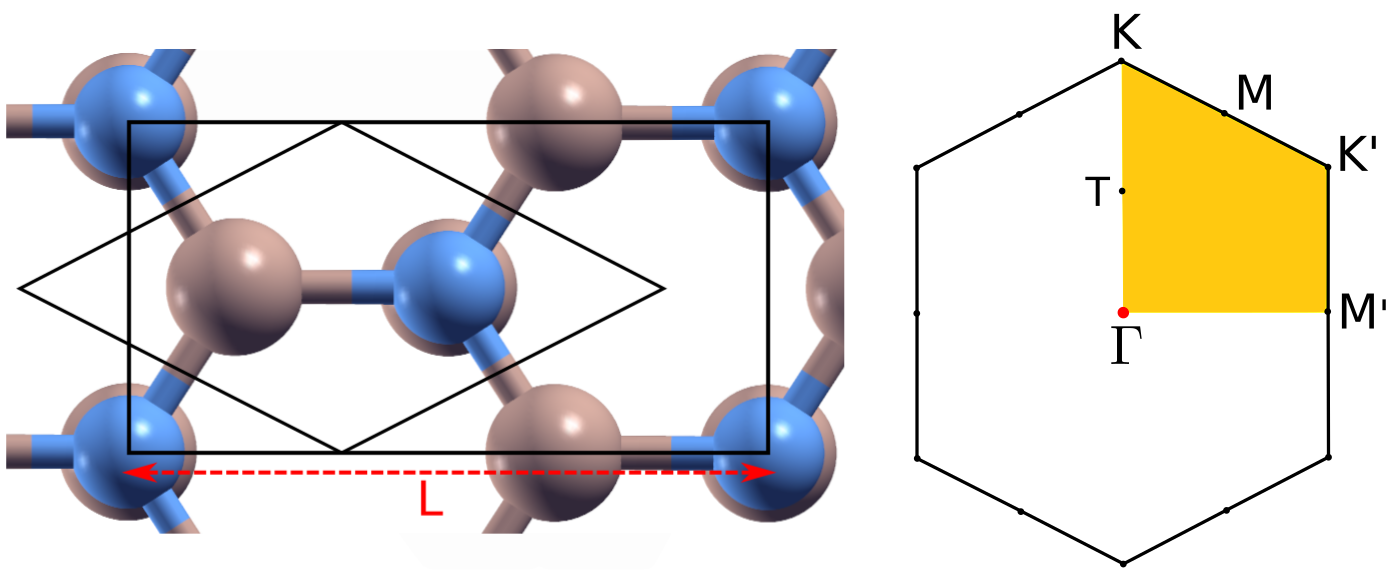
\includegraphics[width=0.5\textwidth]{AppB_structure_BZ.png}
%     \caption{This is Fig. 1 from the main text, put here for convenience.}
% \end{figure}
In our case we a have a crystal with a two-atom basis. We simulate uni-axial strain by elongating or shortening the bond length in only one cartesian direction and letting the atoms relax along the other two orthogonal directions.
It is straightforward to impose such a constraint to a lattice with orthogonal vectors, but more complicated if we had kept the equilibrium hexagonal unit cell. This is why we chose to do the relaxation of structures under strain with orthorombic cells containing 8 atoms (4 per plan).
We want to build a unit cell that preserves the symmetry and periodicity of the strained crystal, with as few atoms as possible. The following is a geometrical generalization of the transformation from orthorombic to hexagonal lattice unit cell in cartesian coordinates.\\
Take an orthorombic unit cell whose matrix in cartesian coordinates is :
\begin{equation}
\begin{pmatrix}
a & 0 & 0\\
0 & b & 0\\
0 & 0 & c
\end{pmatrix}
\end{equation}
with $a,b,c$ being arbitrary lengths.
Now we want to build a strained unit cell that resembles the equilibrium hexagonal cell the most, so that we can compare the different Brillouin zones and the paths on which we plot the electronic structure and the phonon dispersion. The rhombus representing the unit cell of the pseudo-hexagonal cell, viewed from the top, is drawn in Fig. \ref{fig:rhomb}.
\begin{figure}[b]
    \centering
    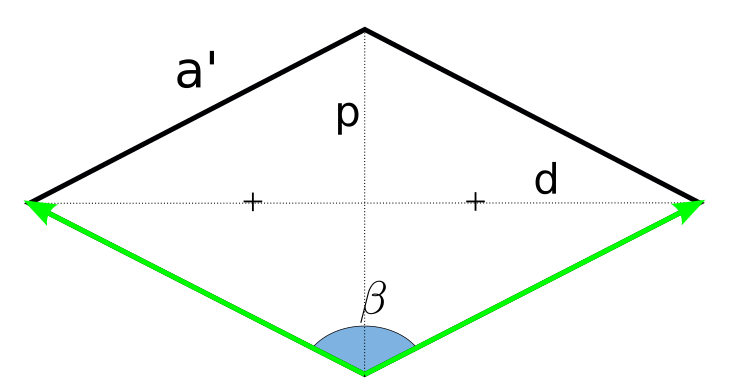
\includegraphics[width=0.5\textwidth]{AppB_rhombus.png}
    \caption{Rhombus used as the unit cell for the pseudo-hexagonal lattice with the atom positions indicated, viewed from top.}
    \label{fig:rhomb}
\end{figure}
Then we have :
\begin{align}
    a' & = \sqrt{d^2 + p^2} \\
    \beta &= \pi - 2 \tan ^{-1} \left(\frac{p}{d}\right)
\end{align}
where $d,p$ are the half diagonals of the rhombus, $a'$ is the side length and $\beta$ the angle as shown in Fig \ref{fig:rhomb}. This is a regular rhombus in the sense that all sides have equal length and the diagonals are orthogonal. The length of the diagonals is obtained from the knowledge of the orthorombic cell, as shown in Fig. \ref{fig:strain_BZ} in the main text.
Then the matrix of this rhombus unit cell, expressed in cartesian coordinates, is :
\begin{equation}
\begin{pmatrix}
a' & 0 & 0\\
a'\cos\beta & a'\sin\beta & 0\\
0 & 0 & c
\end{pmatrix}
\end{equation}
The first two lines are the vectors in green in Fig. \ref{fig:rhomb}. The third vector $c$ is the one perpendicular to the atomic planes and is the same than the orthorombic $c$.
In the equilibrium case, we have $\beta = 120$\textdegree, then this matrix reduces to :
\begin{equation}
\begin{pmatrix}
a' & 0 & 0\\
-a'/2 & a'\sqrt{3}/2 & 0\\
0 & 0 & c
\end{pmatrix}
\end{equation}
which is the standard hexagonal-lattice unit cell. We now have built a 2-atom unit cell which we used to compute electronic, phononic and optical properties of our strained materials. We checked that both the orthorombic and the pseudo-hexagonal unit cells form the same strained crystal when periodically repeated in all directions.